\setchapterpreamble[u]{\margintoc}
\chapter{Funzioni pseudocasuali}
\labch{chapter10}

Vogliamo ora trovare un modo per evitare che nessuno possa modificare il messaggio. Possiamo usare sistemi crittografici non malleabili oppure possiamo aggiungere della ridondanza (codice ciclico, bit di parità). 

Noi vogliamo però costruire dei sistemi che sono resistenti anche da chi tenta di modificare il messaggio in maniera controllata per far quadrare anche il codice di ridondanza. I codici ciclici di ridondanza vengono solitamente usati per proteggerci dall'errore di trasmissione dei dati, che è un errore casuale. 

Vogliamo quindi accodare al messaggio un qualcosa che nessuno riesca a capire se non il reale destinatario finale. Se per esempio scegliessimo al messaggio una funzione casuale (da $k$ bit a $k$ bit) condiviso con l'altra parte, potremmo accodare al messaggio $f(m)$ come \textbf{autenticazione}. In questo modo chi non conosce la funzione casule, che vede solo bit casuali appesi al messaggio, non può modificare in l'autenticazione $f(m)$ del messaggio in modo corretto (lo indovina con probabilità $\frac{1}{2^k}$, con $k$ lunghezza dell'autenticazione).

\section{Generazione di funzioni pseudocasuali}

Sia $U_k$ l'insieme delle funzioni 
\begin{align*}
    U_k: \{0, 1\}^k \rightarrow  \{0, 1\}^k
\end{align*}

\noindent Vogliamo scegliere $f \in_R U_k$. Come facciamo? Generiamo una sequenza di bit pseudocasuali per generare l'indice di $f$ in una enumerazione di $\{0, 1\}^k \rightarrow  \{0, 1\}^k$. L'indice che generiamo è indistinguibile da un indice casuale, e quindi la funzione è come se fosse stata scelta casualmente. 

Questa definizione ha però un problema: la cardinalità di un insieme di funzioni da $A$ a $B$ é $|B|^{|A|}$, quindi 
\begin{align*}
    |U_k| = (2^k)^{(2^k)}
\end{align*}

\noindent Se la cardinalità di questo insieme è $(2^k)^{(2^k)}$, quanti bit ci servono per denotare l'indice di una funzione? I bit che ci servono sono
\begin{align*}
    \log_2 |U_k| = k \cdot 2^k
\end{align*}
\noindent Ci servirebbe una quantità di bit esponenziale, e quindi un tempo esponenziale solo per generare gli indici. Noi vogliamo denotare una funzione usando $k$ bit. Dobbiamo lavorare con un insieme $F_k \subseteq U_k$. Le funzioni che andremo ad usare saranno quindi un sottoinsieme delle possibili funzioni. Vogliamo comunque sceglierle in modo tale che nessuno sia in grado di accorgersi che la funzione sia stata scelta da un insieme più piccolo. 

\begin{definition}[Funzione pseudocasuale]
    Sia $F_k \subseteq U_k$ tale per cui:
    \begin{enumerate}
        \item $|F_k| = 2^k$;
        \item $\exists A \in PPT$ che calcola la seguente funzione:
        \begin{align*}
            i, x \rightarrow f_i(x)
        \end{align*}
        Ogni volta che vogliamo applicare la funzione i-esima all'input $x$, applichiamo un algoritmo polinomiale in grado di farlo;
        \item Sia $D \in PPT$ una macchina che interroga $F$ e ritorna $\{0, 1\}$. Siano
        \begin{itemize}
            \item $P_k^{D, U}$ la probabilità che $D$ restituisca $1$ quando $f \in_R U_k$ (campionata casualmente dall'intero insieme $U_k$);
            \item $P_k^{D, F}$ la probabilità che $D$ restituisca $1$ quando $f \in_R F_k$.
        \end{itemize}
        Allora
        \begin{align*}
            \left| P_k^{D, U} - P_K^{D, F} \right| < k^{-\omega(1)}
        \end{align*}
        Nessuno di coloro che conosce l'indice della funzione deve accorgersi che la funzione è generata (ovvero presa dall'insieme piccolissimo $F_k$).
    \end{enumerate}
\end{definition}

\subsection{Funzione 1}
Siano $G$ un PRSG (Pseudo Random Sequence Generator) e $i$ il seme. Allora il seguente sistema:
\begin{center}
    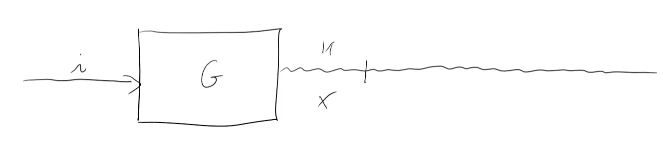
\includegraphics[width=1\textwidth]{images/fun1.png}
\end{center}
\noindent su input $x$ genera $k$ bit, li memorizza e li restituisce. Su un successivo input $y$, se $y = x$ restituisce il risultato precedenti, altrimenti genera altri $k$ bit, li memorizza e li restituisce. In generale, dato un $x$ già usato, $G$ ritorna i $k$ bit associati.

Questo è un generatore di bit pesudocasuali? Supponiamo che Alice e Bob vogliano scambiarsi dei messaggi autenticati ($m, f(m)$) con questo sistema. Entrambi conoscono il seme $i$ da passare al generatore di funzioni pseudocasuali. Se la comunicazione è sequenziale, come in figura \ref{fig:fun1-1}, il sistema funziona correttamente in quanto l'ordine in cui vengono generate le sequenze di $k$ bit è la stessa per Alice e Bob. 
\begin{figure}
    \centering
    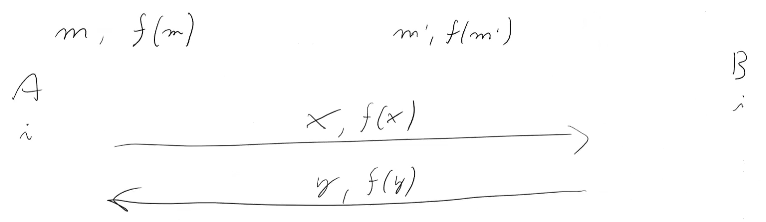
\includegraphics[width=1\textwidth]{images/fun1-1.png}
    \caption{Alice invia un messaggio, Bob lo verifica, Bob risponde, Alice verifica la risposta.}
    \label{fig:fun1-1}
\end{figure}

Se invece Alice e Bob inviano ciascuno un messaggio all'altro contemporaneamente, i messaggi non vengono autenticati \ref{fig:fun1-2}. Il sistema descritto associa la prima sequenza di bit al primo input passato, la seconda al secondo (se diverso da quello già memorizzato) e così via. Quindi il sistema di Bob assocerà la prima sequenza a $y$, mentre quello di Alice a $x$, rendendo così errata l'autenticazione. 
\begin{figure}
    \centering
    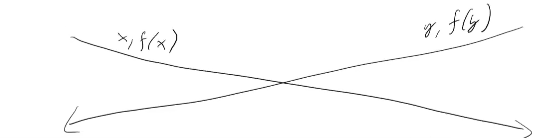
\includegraphics[width=1\textwidth]{images/fun1-2.png}
    \caption{Alice invia un messaggio, Bob invia un messaggio, Bob verifica, Alice verifica.}
    \label{fig:fun1-2}
\end{figure}

\noindent Questo sistema potrebbe essere usato quando esiste un repository centralizzato. Inoltre, necessita di un database che mantenga tutte le richieste già effettuate; maggiore sono le entry, più tempo è necessario a ottenere una risposta dalle interrogazioni.

Questo sistema non soddisfa la nostra definizione di funzioni pseudocasuali in quanto $F_k$ non è un insieme ben definito.

\subsection{Funzione 2}
Siano $G$ un PRSG (Pseudo Random Sequence Generator) e $i$ il seme. Dato il seguente sistema
\begin{center}
    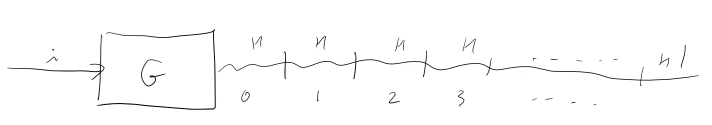
\includegraphics[width=1\textwidth]{images/fun2.png}
\end{center}

\noindent dividiamo l'output di $G$ in tanti gruppi di $k$ bit ciascuno. Associo il primo gruppo a $f_0$, il secondo a $f_1$, il terzo a $f_3$ e così via. Allora 
\begin{align*}
    f_i(x) = \text{ x-esimo gruppo di $k$ bit restituito da $G$}
\end{align*}

\noindent Con questo sistema l'insieme $F_k$ è ben definito e la sua cardinalità è $|2^k|$. La seconda proprietà è verificata? No, non esiste alcun algoritmo $A \in PPT$ che soddisfi al proprietà.
\begin{proof}
    Sia $x$ una sequenza di $k$ bit a $1$, ovvero:
    \begin{align*}
       x = 1 \ .... \ 1 = 2^{k}-1
    \end{align*}
    \noindent Per calcolare $f_i(x)$, dobbiamo prendere il gruppo in posizione $2^k-1$. Per come è definito un generatore id bit pseudocasuali, per calcolare questo gruppo dobbiamo generare tutti i bit che vengono prima, che sono $k \cdot 2^k$ bit. Ci serve un tempo esponenziale.
\end{proof}

\subsection{Funzione 3}
Siano $G$ un PRSG (Pseudo Random Sequence Generator) e $i \oplus x$ il seme. Dato il seguente sistema:
\begin{center}
    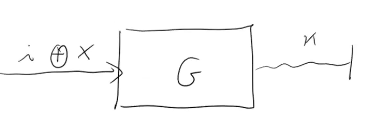
\includegraphics[width=0.8\textwidth]{images/fun3.png}
\end{center}

\noindent prendiamo solo i primi $k$ bit come risultato. Allora:
\begin{align*}
    f_i(x) = \text{ primi $k$ bit di $G$ con seme $i \oplus x$}
\end{align*}

\noindent Verifichiamo se rispetta le tre proprietà:
\begin{enumerate}
    \item L'insieme ha cardinalità $|2^k|$ e l'indice $i$ definisce in maniera univoca la funzione ($f_i(x)$ è ben definita);
    \item La funzione $f_i(x)$ è calcolabile polinomialmente;
    \item Supponiamo per assurdo che esiste $D$ tale per cui:
    \begin{align*}
            \left| P_k^{D, U} - P_K^{D, F} \right| > k^{-\omega(1)}
        \end{align*}
    Abbiamo quindi una macchina PPT che vede la differenza. Vorremmo trasformare $D$ in macchina che attacca il generatore $G$, ovvero che ci permette di violare la sicurezza di $G$ (che permette di distinguere sequenze di bit pseudocasuali da realmente casuali oppure permette di predire il bit successivo). 
    Per farlo dobbiamo prendere il distinguisher $D$ e vedere gli esperimenti che questo fa sulla funzione $f$ come esperimenti che noi facciamo sul generatore $G$. Se gli esperimenti che facciamo sono compatibili, ovvero soddisfano tutti i vincoli che abbiamo dato nel definire la correttezza di un generatore di bit pseudocasuali, possiamo vedere $D$ come un distinguisher per il generatore $G$.

    Affinché $D$ sia veramente un distinguisher che ci permetta di vedere qualcosa di interessante sul generatore $G$, è importante che gli esperimenti che $D$ sta facendo implicitamente su $G$ passando per $f$ siano compatibili con gli esperimenti che un distinguisher sta facendo su $G$ quando diciamo che $G$ non è distinguibile.

    Se riprendiamo la definizione di generatore di bit pseudocasuali, l'esperimento che si fa è il seguente: 
    \begin{itemize}
        \item Genera un seme a caso, usa il seme per generare una sequenza e fa osservare a $D$ la sequenza generata. $D$ deve cercare di dire qualcosa;
        \item Genera un altro seme a caso, usa il seme per generare una sequenza e fa osservare a $D$ la nuova sequenza generata. $D$ deve cercare di dire di nuovo qualcosa;
        \item E così via.
    \end{itemize}
    A $D$ possiamo far vedere un numero qualsiasi di sequenze, ma gli esperimenti che $D$ può fare devono essere esperimenti indipendenti. 
    
    Nel caso specifici della funzione 3, il distinguisher può scegliere valori diversi di $x$ (può interrogare $f$ su $x_1$, $x_2$, ...), ma il generatore $G$ conosce $x_1$, $x_2$, ... . Se prendiamo lo XOR tra 2 degli input usati da $G$, otteniamo lo XOR del seme che è stato usato da $G$ per generare $f_i(x)$. Il nostro distinguisher può fare diversi esperimenti dove va a controllare $k$bit generati da $G$, ma a differenza della nostra definizione di bit pseudocasuali, il nostro distinguisher è in grado di osservare l'output di $G$ su 2 semi di cui è nota la differenza.

    Se ad esempio interroghiamo $f(0) = a$ e $f(1^k) = b$, sappiamo che il seme usato per generare $a$ è il complemento del seme usato per generare $b$. Il seme usato per $f(0)$ è esattamente $i$, mentre il seme usato per $f(1^k)$ è il complemento di $i$. In generale se interroghiamo $f(x) = a'$ e $f(y) = a''$, lo XOR dei semi usati per generare $a'$ e $a''$ è $x \oplus y$. 

    Gli esperimenti che il distinguisher $D$ riesce a fare implicitamente su $G$ sono esperimenti che il distinguisher che abbiamo usato per definire la correttezza di $G$ non è in grado di fare. Quindi il distinguisher che sta lavorando sulle funzioni pseudocasuali è più potente del distinguisher che abbiamo ammesso nella definizione di correttezza di un generatore di bit pseudocasuali. I casi sono due:
    \begin{itemize}
        \item Abbiamo definito un generatore di bit pseudocasuali troppo debole e quindi ci serve una definizione più forte che ammetta anche esperimenti di questi tipo, oppure possiamo dimostrare che il generatore che abbiamo definito resiste anche agli attacchi che questo $D$ è in grado di fare;
        \item  Non vediamo alcun vantaggio che l'attaccante possa trarre da questo tipo di esperimento più potente e quindi lo teniamo "buono".
    \end{itemize}

    In crittografia bisogna sempre essere scettici: se non vediamo un modo  in cui si riesca a rompere qualche cosa non significa che qualcun altro possa trovarlo. 

    In questo caso è possibile costruire un generatore $G$, che è un generatore di bit pseudocasuali, che costruito in questo contesto permette effettivamente di costruire un distinguisher. Nel momento in cui siamo in grado di farlo, questa dimostrazione non potrà mai funzionare, ovvero non si potrà mai partire di un distinguisher $D$ per il generatore di funzioni pseudocasuali e costruire un distinguisher per il generatore di bit pseudocasuali.

    Costruiamo ora un generatore di bit pseudocasuali che in questo contesto è distinguibile. 

    Supponiamo di avere un generatore $G$ che prende in input $k-1$ bit e produce la sequenza pseudocasuale. Il generatore è contenuto in una macchina $G'$ che prende un seme $i$ di $k$ bit. La nostra richiesta è di produrre un generatore che prende in input $k$ bit, ma noi ne abbiamo a disposizione solo uno a $k-1$ bit. Allora procediamo così:
    \begin{itemize}
        \item Dato il seme $i = i_0 \ i_1 \ ... \ i_{k-1}$ di $k$ bit, usiamo il bit $i_0$ some selettore;
        \item Se $i_0 = 0$, allora ritorniamo:
        \begin{align*}
            G(i_1 \ ... \ i_{k-1})
        \end{align*}
        \item Se $i_0 = 1$, allora ritorniamo:
        \begin{align*}
            G(\overline{i_1 \ ... \ i_{k-1}})
        \end{align*}
    \end{itemize}
    Poiché il complemento di una sequenza casuale resta una sequenza casuale, stiamo producendo sequenza pseudocasuali di bit con seme da $k-1$ bit in entrambi i casi. $G$ prende sempre in input una sequenza di bit casuali che è generata uniformemente tra i gruppi di $k-1$ bit: con probabilità $\frac{1}{2}$ il seme è la sequenza casuale originale generata, con probabilità $\frac{1}{2}$ è il suo complemento. L'output di $G'$ è l'output di un seme distribuito uniformemente tra tutti i semi. Quindi $G'$ si comporta esattamente come $G$, anche se prende in input un bit in più. 
    Tuttavia se questo oggetto lo usiamo nel contesto sopra scopriamo che $f(0)$ e $f(1^k)$ sono la stessa cosa: 
    \begin{itemize}
        \item se con $f(0)$ generiamo il seme $i_0 \ i_1 \ ... \ i_{k-1}$, con $i_0 = 0$, allora
        \begin{align*}
            G' = G(i_1 \ ... \ i_{k-1})
        \end{align*}
        \item Di conseguenza, $f(1^k)$ genererà il seme $\overline{i_0 \ i_1 \ ... \ i_{k-1}}$, con $\overline{i_0} = 1$, e quindi:
        \begin{align*}
            G' = G(\overline{\overline{i_1 \ ... \ i_{k-1}}}) = G(i_1 \ ... \ i_{k-1})
        \end{align*}
    \end{itemize}
    
    Il distinguisher diventa una macchina banale:
    \begin{itemize}
        \item Calcola $f(0)$ e $f(1^k)$;
        \item Se sono uguale ritorna $1$;
        \item Se sono diversi ritorna $0$.
    \end{itemize}
    Questo distinguisher di fronte ad una funzione pseudogenerata rispenderà sempre $1$, di fronte ad una funzione casuale risponderà $1$ solo quando $f(0) = f(1^k)$, ovvero con probabilità $\frac{1}{2^k}$.

    Questa costruzione, nonostante sia stupida, è permessa dalla nostra definizione di generatore pseducasuale.
\end{enumerate}

\subsection{Funzione 4}

Torniamo alla funzione 2:
\begin{center}
    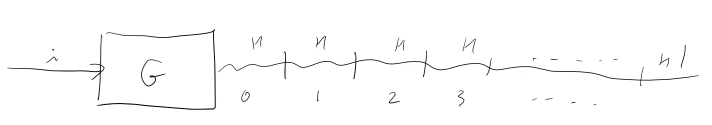
\includegraphics[width=1\textwidth]{images/fun2.png}
\end{center}

\noindent dividiamo l'output di $G$ in tanti gruppi di $k$ bit ciascuno. Associo il primo gruppo a $f_0$, il secondo a $f_1$, il terzo a $f_3$ e così via. Allora 
\begin{align*}
    f_i(x) = \text{ x-esimo gruppo di $k$ bit restituito da $G$}
\end{align*}

\noindent Per poter calcolare $f_i(x)$ in PPT usiamo un generatore BBS (Blum Blum Shoup). Quando lavoriamo col logaritmo discreto non siamo in grado di calcolare elemente troppo distanti, ma se dobbiamo calcolare:
\begin{align*}
    f_i(2^k - i) = \text{ bit dalla posizione $k\cdot (2^k-1)$ a $k \cdot 2^k$}
\end{align*}

\noindent Come facciamo? Dobbiamo prendere
\begin{align*}
    i^{2^{(2^k-1)-1}}
\end{align*}

\noindent Questo esponenziale sembra complicato da calcolare. Tuttavia sappiamo che gli esponenti lavorano modulo $\varphi(n)$, quindi stiamo calcolando un esponente modulo $\varphi(n)$:
\begin{align*}
    i^{2^{(2^k-1)-1 \pmod{\varphi(n)}}}
\end{align*}

\noindent Questo lo sappiamo calcolare con l'iterative squaring. Una volta calcolato l'esponente possiamo calcolare l'esponenziale modulo $\varphi(n)$ in tempo polinomiale:
\begin{align*}
    i^{2^{(2^k-1)-1 \pmod{\varphi(n)}}} \pmod{\varphi(n)}
\end{align*}

\noindent Di conseguenza questo oggetto è calcolabile in PPT, quindi disponiamo di un $A$ che calcola $f_i(x)$ in tempo polinomiale. Non possiamo fare questo con ogni generatore, ma solo con BBS riusciamo ad ottimizzare le operazione e calcolare direttamente un bit senza calcolare quelli precedenti. 

\noindent A questo punto disponiamo di un generatore $G$ che rispetta i punti 1 e 2. Vediamo ora se rispetta anche il punto 3.

Supponiamo di avere un distinguisher che interroga $f$, facendo ovviamente implicitamente degli esperimenti su $G$ (genera un seme, guarda alcuni gruppi a caso - $0, 1, 5, 2^k-1$ -). Il distinguisher che stiamo usando qui ha la stessa potenza del distinguisher usato nella definizione di $G$? Quando parliamo di esperimenti su $G$, generiamo una sequenza di bit di una data lunghezza e andiamo a guardarla, quindi generiamo tutti i bit. In questo caso possiamo generare una sottosequenza di bit senza generare i bit che la precedono (possiamo generare il gruppo 4 senza generare i primi 3). Potremmo quindi anche andarci bene, in quanto vedere solo un gruppo è "peggio" che vedere un gruppo e quelli che lo precedono.

Il problema è che il nostro distinguisher può vedere anche il gruppo $2^k-1$ come una sequenza polinomiale di bit, mentre il distinguisher per $G$ vedrebbe $2^k-1$, più tutta la sequenza precedente, come una sequenza esponenziale. Noi non permettiamo ad un algoritmo polinomiale di vedere una sequenza esponenziale, di conseguenza $D$ è in grado di vedere dei bit che il distinguisher per $G$ non potrebbe mai vedere. Se quei bit li fossero quelli utili a capire se ci troviamo di fronte a un generatore di bit pseudocasuali o no, per la definizione di $G$ questi non sarebbero un problema perchè il distinguisher non li vedrebbe mai. Con $D$ però siamo in grado di vedere questi bit, quindi l'esperimento che stimo facendo con $D$ non può essere tradotto in un esperimento contro il generatore $G$. 

Come facciamo a concludere che l'esistenza di un distinguisher per le funzioni implica l'esistenza di un distinguisher per un generatore, quando questo distinguisher sta facendo cose che non potrebbero essere mai fatte su $G$? Non possiamo farlo.

In generale i crittografi, se non trovano una dimostrazione di correttezza per un sistema, tendono a scartarlo, a meno che non ve ne siano altri usabili. 

\subsection{Funzione 5}
Partiamo da un seme $s = i$ e usiamo usiamo un generatore $G$ per generare $G(s)[0\ ...\ k-1]$ (generatore per i bit $\ ...\ k-1$) e usiamo lo stesso generatore per generare $G(s)[k \ ...\ 2k-1]$. Stiamo usando il generatore $G$ per generare $2k$ bit: i primi $k$ bit li posizioniamo a sinistra, i restanti a destra. Chiamiamo il ramo di destra 0 e il ramo di sinistra 1. Chiamiamo i due semi che abbiamo generato $s_0$ e $s_1$.
\begin{center}
    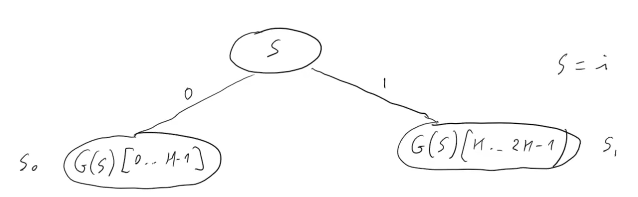
\includegraphics[width=1\textwidth]{images/fun5-1.png}
\end{center}

\noindent Aggiungiamo un altro livello. 
\begin{center}
    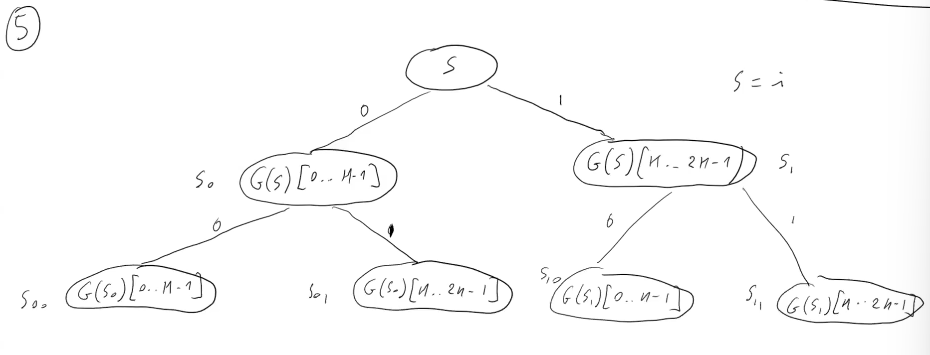
\includegraphics[width=1\textwidth]{images/fun5-2.png}
\end{center}

\noindent Ripetiamo il procedimento fino ad arrivare al nodo $s_x$.
\begin{center}
    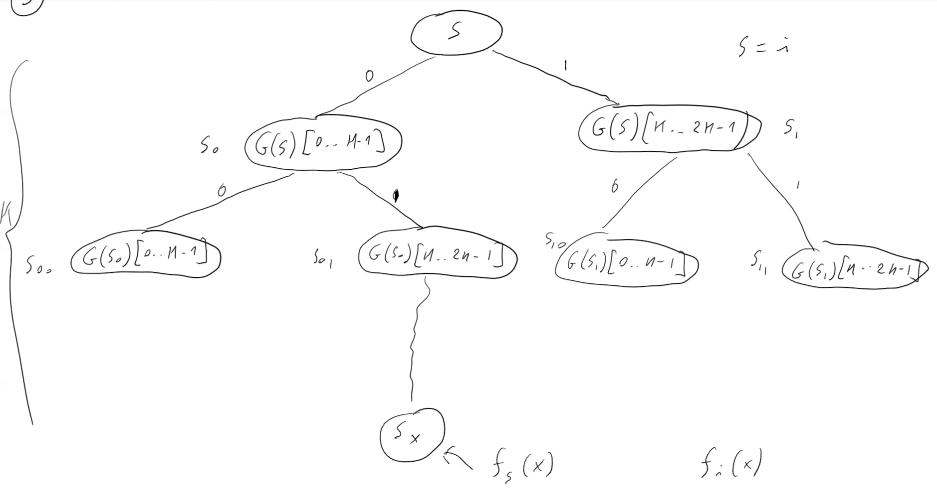
\includegraphics[width=1\textwidth]{images/fun5-3.png}
\end{center}

\noindent Siamo scesi per $k$ livelli, arrivando a nodi dove i semi sono indicizzati da $k$ bit. Il seme indicizzato da $x$ è $f_s(x)$, cioè $f_i(x)$, in quanto abbiamo ridenominato $i$ in $s$. 

Abbiamo costruito un albero di profondità $k$ e abbiamo scoperto come costruire i nodi di questo albero. L'albero ha $2^k$ nodi. Le foglie rappresentano i valori della funzione sui vari argomenti, a partire dal seme $s$ messo in radice. 

Dato $s$ la funzione è ben $f_s$ definita (costruiamo l'albero e andiamo a prendere la foglia di indice $x$). Esiste un algoritmo PPT in grado di calcolare $f_s(x)$? Per calcolare $f_s(x)$ non è necessario calcolare tutto l'albero, ma basta seguire il percorso da $s$ verso $s_x$. Per ogni livello generiamo massimo $2k$ bit per $k$ bit. Il generatore BBS, per generare un bit fa un elevamento al quadrato. Se deve costruire $2k$ bit, fa $2k$ volte un elevamento al quadrato. Quindi per ognuno dei $2k$ bit deve fare un elevamento al quadrato, che corrisponde ad una moltiplicazione che costa $k^2$. Quindi la complessità totale è:
\begin{align*}
    k \cdot 2k \cdot k^2 = \Theta(k^4)
\end{align*}
 \noindent Quindi l'algoritmo $A$ PPT che calcola $f_s(x)$ esiste. \\

 \noindent Vediamo ora il punto 3. Che tipo di esperimenti stiamo facendo implicitamente su $G$? Stiamo usando $G$ su un insieme di semi che non sono casuali, ma nidificati. L'uso nidificato delle funzioni, tuttavia, risulta migliore rispetto all'uso sequenziale o su argomenti in relazione tra di loro. 

 Ci troviamo ad un dato livello, e da quello stimo passando al successivo (dal livello 1 al livello 2, dal 2 al 3 e così via). Noi potremmo guardare questo albero per livelli. Un generatore pseudocasuale trasforma una certa quantità di casualità in una quantità di casualità diversa. Il nostro generatore lavora da un livello al successivo. Se riuscissimo a ricondurci ad un albero dove stiamo generando le funzioni pseudocasuali, ma in qualche modo ci concentriamo sul passaggio da un livello al successivo, allora siamo in un contesto dove stiamo lavorando con un generatore di bit pseudocasuali classico. 

 Per ogni livello $i = 0 \ ... \ k$ definiamo l'albero $T_i$ tale che:
 \begin{enumerate}
     \item I nodi dei livelli $0 \ ... \ i$ sono tutti casuali;
     \item I nodi dei livelli $i+1 \ ... \ k$ sono generati dai livelli precedenti.
 \end{enumerate}

\noindent Nel nostro albero la radice è casuale, mentre ogni altro nodo è stato generato ognuno a partire dal livello precedente. 

Abbiamo $T_0$ dove $s$ è random e il resto è pseudogenerato, $T_k$ dove tutto è random, $T_i$ dove fino al livello $i$ è random e il resto è generato.
\begin{center}
    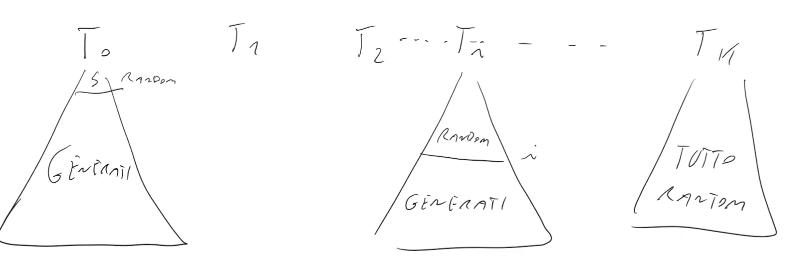
\includegraphics[width=1\textwidth]{images/fun5-4.png}
\end{center}

\noindent Definiamo $H_i$ la funzione costruita da un albero $T_i$ (vogliamo calcolare una funzione, per farlo costruiamo un albero $T_i$ e abbiamo una funzione campionata da $T_i$). LO schema $T_0$ è uno schema dove la radice è casuale e tutto il resto è generato. Un albero costruito secondo questo schema è esattamente l'albero che abbiamo costruito nella funzione 5. Un albero $T_k$ tutti i nodi sono veramente casuali, per calcolare $f_x$ andiamo a guardare la foglia $x$ che è scelta in maniera veramente casuale. Un albero costruito secondo lo schema $T_k$ rappresenta una funzione campionata da $U_k$. L'albero $T_0$ rappresenta una funzione campionata da $F_k$.

Lo schema i-esimo è un modo per generare funzioni pseudocasulae dove, anziché usare come seme solo il livello 0, usiamo come semi tutti i livelli fino al livello i-esimo. Sono $k+1$ modi diversi per generare una funzione pseudocasuale.

Definiamo come $P(i)$ la probabilità che $D$ restituisca $1$ quando interagisce con una funzione geenrata secondo lo schema $T_i$. Possiamo scegliere come generare una funzione pseudocasuale con ognuno di questi schemi. Scelto lo schema, possiamo generare una funzione che lo segue, darla in pasto a $D$ e verificare con che probabilità ritorna $1$. A questo punto è chiaro che:
\begin{align*}
    P(0) = P_k^{D, G} \hspace{2cm} P(k) = P_k^{D, U}
\end{align*}

\noindent Supponiamo che il nostro distinguisher distingua, ovvero:
\begin{align*}
    \left|P_k^{D, G} - P_k^{D, U} \right| > k^{-c} = \left|P(0) - P(k) \right| > k^{-c}
\end{align*}

\noindent Possiamo lavorare ora a livello di interpolazione:
\begin{align*}
    \exists i \ \left| P(i) - P(i+1) \right| > k^{-c'}
\end{align*}

\noindent Abbiamo visto che gli schemi estremi sono quelli su cui abbiamo le ipotesi. Se abbiamo la capacità di distinguere due schemi estremi allora abbiamo anche la capacità di distinguere due schemi adiacenti. Se prendiamo gli schemi $T_i$ e $T_{i+1}$, nel primo caso il livello $i+1$ è generato dal livello $i$, nel secondo caso è causale. Quindi se confrontiamo i due schemi, l'unica differenza che troviamo sta nel livello $i+1$. Con il nostro $G$ non facciamo altro che andare a fare dei test sui bi del livello $i+1$.

Quali sono i test che stiamo facendo su questo livello? Quando chiediamo $G(x)$, andiamo indietro e prendiamo un nodo specifico al livello $i+1$, non stiamo facendo altro che fare dei calcoli che ci portano a vedere $x$, non vediamo tutti i calcoli intermedi (il distinguisher $D$ non vede nodi tra il fondo e $x$), anche se il generatore li genera. Delle cose che possiamo costruire a partire da un nodo del livello $i+1$ vediamo solo una parte.

Non è un problema vedere meno di quello che un distinguisher su un generatore $G$ può vedere. Il punto è che se calcoliamo $f_x$ su $T_{i+1}$, stiamo praticamente dicendo di generare dei bit casuali di partenza e di fare delle elaborazioni per ottenere $x$; se lo stiamo facendo sull'albero $T_i$ stiamo dicendo di generare dei bit casuali, generare un seme, usare il seme per generare dei bit da usare per calcolare $x$. Il nostro esperimento sta lavorando, in un caso, su bit veramente casuale, nell'altro sta lavorando su un seme casuale usato per generare dei bit per arrivare a $x$.

E se chiediamo una $y$ che fa riferimento allo stesso nodo? Questo si traduce nello stesso identico esperimento sul livello $i+1$, quindi non è un esperimento nuovo, abbiamo fatto due calcoli a partire dalla stessa osservazione fatta. E se lavoriamo su una $z$ che va su un nodo diverso? In questo caso stiamo facendo un nuovo esperimento su $G$, dove stiamo lavorando con altri bit casuali o generato. I bit generati vengono però generati a partire da un altro seme che è indipendente dal precedente. I semi sono indipendenti; una volta che abbiamo definito gli argomenti $x_1, x_2, x_3, ...$, risalendo troviamo un insieme di nodi, ma tutto ciò che parte dai nodi e scende è un esperimento indipendente dagli altri. Il test che stiamo facendo su $f$ è un test che stiamo facendo sul livello i-esimo per capire se è casuale o generato, ed è fatto nella forma corretta che era stata prevista quando abbiamo definito i generatori di bit pseudocasuali $G$. 

Questo ci dimostra che un eventuale attaccante a un generatore di funzioni si traduce in un eventuale attaccante a un generatore di bit pseudocasuali, e di conseguenza un distinguisher non esiste se partiamo dalla definizione di $G$ che abbiamo dato.

\noindent\fbox{%
    \parbox{\textwidth}{%
    Se noi prendiamo un nodo del livello $i-1$ e prendiamo tutto il suo albero, tutto le interrogazioni che facciamo lì sotto, sono in realtà interrogazione su $2k$ bit generati a partire dal livello precedente. Per noi sono un esperimento unico, perché effettivamente l'esperimento che facciamo parte dal generatore e calcola tutto ciò che vuole. Noi vediamo il livello $i+1$ pseudogenerato o veramente casuale, e facciamo degli esperimenti mirati a calcolare della roba che viene sotto. Questo è ciò che fa il distinguisher, e questo distinguisher può fare l'esperimento più volte, ma sono tutti esperimenti indipendenti in quanto ciascun seme è generato in maniera indipendente (è come usare il distinguisher per il singolo bit più volte, a differenza degli altri casi dive utilizzavamo i distinguisher su semi che conoscevamo, oppure facevamo esperimenti che non si potevano fare in tempo polinomiale)
    }
}

\\\\



Siamo partiti dalla generazione di bit pseudocasuali. Da questa dopo aver trovato un sistema dimostrabilmente sicuro siamo passati alla generazione di funzioni pseudocasuali. Una funzione pseudocasuale è una scatola nera che contiene una funzione che possiamo interrogare con argomenti che ottenere risposte. La funzione è scelta casualmente fra tutte le funzioni tra $k$ bit a $k$ bit. In realtà la funzione non è scelta tra tutte le funzioni ma tra un insieme ristretto, in quanto dobbiamo denotare questa funzione con un insieme di $k$ bit. L'indice scelto determina la funzione da usare.  

Se i $k$ bit vengono scelti a caso, la cardinalità dell'insieme in cui scegliamo le funzioni è $2^k$. Questo generatore funziona bene nella misura in cui chi interagisce con la scatola nera non capisce se questa sta calcolando una funzione scelta dall'insieme grande o da quello ristretto. 

Visto che la scatola nera la dobbiamo costruire, vogliamo che dato, indice e argomento, in tempo probabilistico polinomiale sia possibile calcolare $f_i(x)$. Abbiamo provato varie soluzioni, di cui abbiamo sempre trovato qualche difetto. 





